\chapter{Linear regulation}
\section{Theory and related work} \label{sec:literature_linear}
A linear regulator is a device that uses a closed feedback loop to continuously adjust a voltage divider network to maintain a constant output voltage. The main drawback of this regulation topology is that efficiency is limited as the difference between the input and output voltage is dissipated as heat.

\section{Design} \label{sec:design_linear}
For the purpose of this design a MC78L05 was chosen, since this regulator could handle up to $\SI{35}{V}$ input voltages it was compatible with the maximum $\SI{12}{V}$ output from the intermediary voltage stage. To ensure that the integrated chip could handle the required power requirements the necessary heat sink calculations needed to be completed. \newline 
Given these design requirements a $\SI{7}{V}$ difference was induced across the input and output of the regulator, and a maximum output current of $\SI{40}{\milli A}$ was chosen, which was less than the $\SI{100}{\milli A}$ current the regulator can supply. Furthermore under these conditions a power dissipation of $\SI{280}{\milli W}$ can be expected, which is much less than the $\SI{750}{\milli W}$ maximum power dissipation the regulator is designed for \cite{reg78L05:2002}. By applying Equation \ref{eq:mc78l05temp} from \cite{Perold:2019} and choosing an ambient temperature of $\SI{25}{\degree C}$, the maximum induced temperature was found to be $\SI{67}{\degree C}$, which is far below the maximum allowable operating temperature of $\SI{150}{\degree C}$.\newline
\begin{equation}
   T_{max} = P_{max}(R_{\Theta _{JA}}) + T_{A}
   \label{eq:mc78l05temp}
\end{equation}
Referring to Figure \ref{fig:5vregulator} the capacitor C1 had to be added to the circuit if the regulator was far away from the power supply filter and served the purpose of rejecting attenuation and specifically AC noise. The capacitor C3 was added to the output of the regulator in order to improve stability and to improve the regulators transient response, both of these capacitors were chosen according to datasheet recommendations.

\begin{figure}
    \centering
    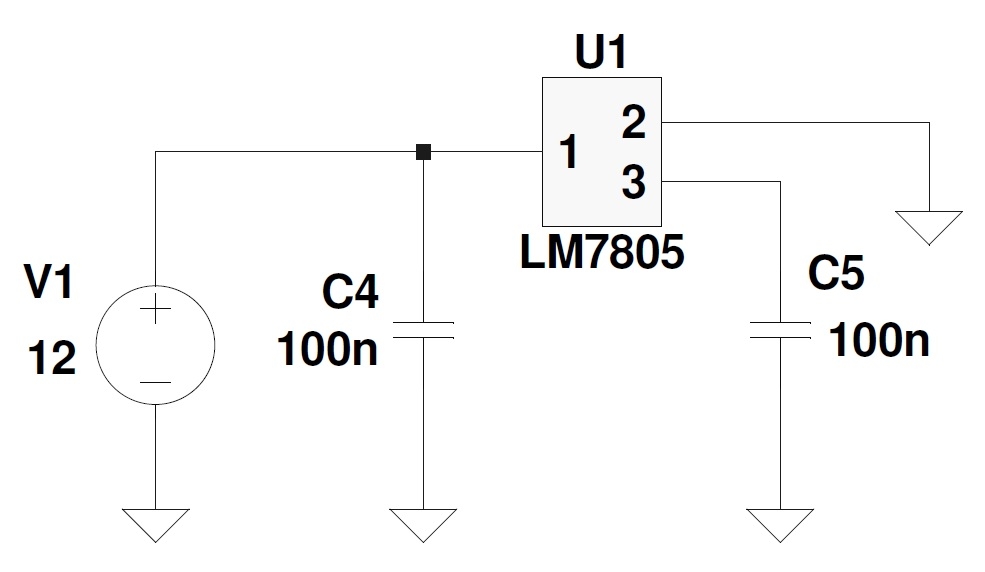
\includegraphics[width = 0.45\linewidth]{Figures/linearreg.jpg}
    \caption{Circuit schematic of the 5V regulator}
    \label{fig:5vregulator}
\end{figure}

\section{Simulation} \label{sec:simulation_linear}
In order to see if the designed circuit operated as required it was simulated in SPICE. The circuit was tested over a various range of load resistor values to see how much power was being consumed and to see if the output voltage remained stable.\newline
These results were listed in Table \ref{tab:linearregtable}, and as can be seen in the last column the power dissipated by the linear regulator was much higher than initially calculated. However this is not a problem as the maximum load requirements do not exceed the maximum power ratings of the linear regulator, and the regulator does not get hot enough to require a heat sink.

\begin{table}
        \centering
        \footnotesize
        \caption{Table showing simulated power consumption of linear regulator.}
         \begin{tabular}{c@{\qquad}rrrr}
          \toprule
           Load Resistance ($\Omega$) & Output Voltage ($\SI{}{V}$) & Power ($\SI{}{\milli W}$) \\
           \midrule
            No load     & 5.0028     & 60.80  \\
            1k          & 5.0028     & 95.72  \\
            470         & 5.0028     & 135.18  \\
            280         & 5.0028     & 185.70 \\
            Full load (125) & 5.0028 & 340.8 \\
          \bottomrule
        \end{tabular}
     \label{tab:linearregtable}
\end{table}

\section{Measurements} \label{sec:measurements_linear}
The measured output voltage of the regulator was found to be $\SI{5.14}{V}$ under no load conditions, and $\SI{5.12}{V}$ under full load conditions supplying $\SI{40}{\milli A}$ as shown in Figure \ref{subfig:5V_reg_output}. This was $2.8\%$ higher than was designed for but still within a acceptable $5\%$ tolerance. As can be seen in Figure \ref{subfig:5V_reg_noise} a noise level of less than $\SI{10}{\milli V}$ peak to peak was measured on the $\SI{5}{V}$ rail, which confirms that the regulator meets all the required specifications. \newline
Furthermore from \cite{reg78L05:2002} it was found that the regulator had a maximum quiescent current of $\SI{5.5}{\milli A}$, given this and a load of $\SI{120}{\Omega}$ the expected efficiency of the regulator was calculated as $37.3\%$ using Equation \ref{eq:efficiency}.

\begin{equation}
   \eta = \frac{P_{out}}{P_{in}}
   \label{eq:efficiency}
\end{equation}

\begin{figure}
 \centering
     \begin{subfigure}[]{0.45\textwidth}
        \centering
         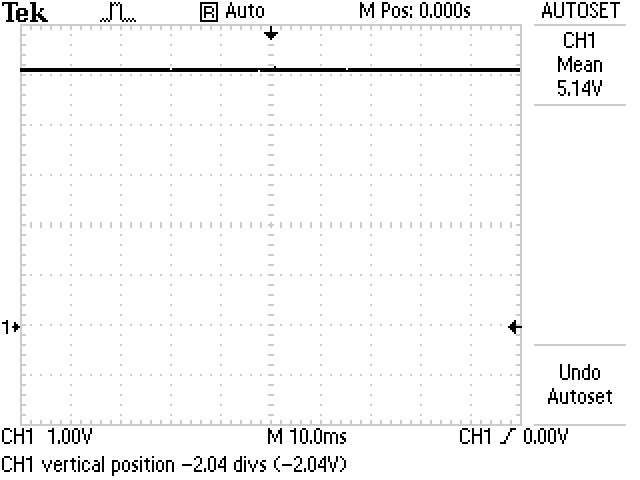
\includegraphics[width=1\linewidth]{./Figures/5V_output_voltage.JPG}
		    \caption{Linear regulator output} \label{subfig:5V_reg_output}
     \end{subfigure}
      \begin{subfigure}[]{0.45\textwidth}
              \centering
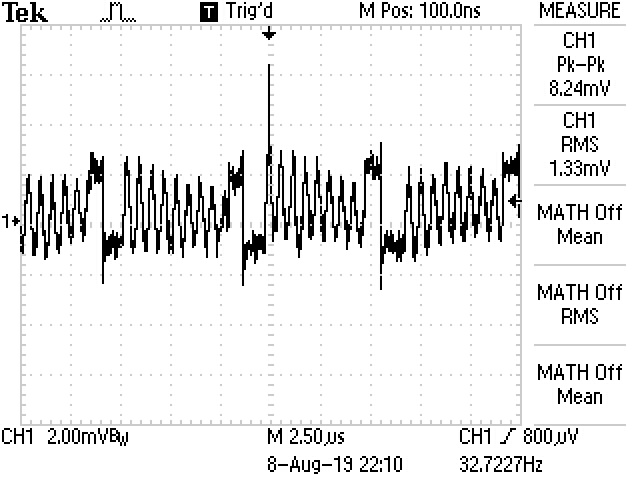
\includegraphics[width=1\linewidth]{./Figures/5V_output_noise.JPG}%
		    \caption{Noise characteristics}  \label{subfig:5V_reg_noise}
     \end{subfigure}
   \caption[Measured 5V Regulated Output Voltage Plots]{Measured 5V Regulated Output Voltage Plots. (a) reading showing output voltage, (b) output noise of the regulator}
    \label{fig:regulator_simulation_results_box}
 \end{figure}







